\chapter{Programme \texttt{FCC}}

\section{Présentation du Projet FCC}

Le FCC (Futur Collisionneur Circulaire) est le projet du CERN pour remplacer 
leur collisionneur actuelle, le LHC (Large Hadronic Collider). 
Dont la fin de l'exploitation est prévu en 2040 \cite{cern:fcc}.
On prévoit un anneau de 100 km, contre 27 km pour le LEP et le LHC 
(comme montrer Figure~\ref{fcc:img}).
Ce qui devrait nous permettra d'atteindre une énergie de 100 $\TeV$ contre 13 $\TeV$
actuellement pour le LHC.

L'objectif est la rechercher d'une nouvelle physique par la mise en évidence de déviation avec le modèle standard. Et plus particulièrement, en augmentant la statistique sur le boson de Higgs, découvert avec le collisionneur actuelle, afin de mieux comprendre sa physique.

\begin{figure}[!ht]
    \centering
    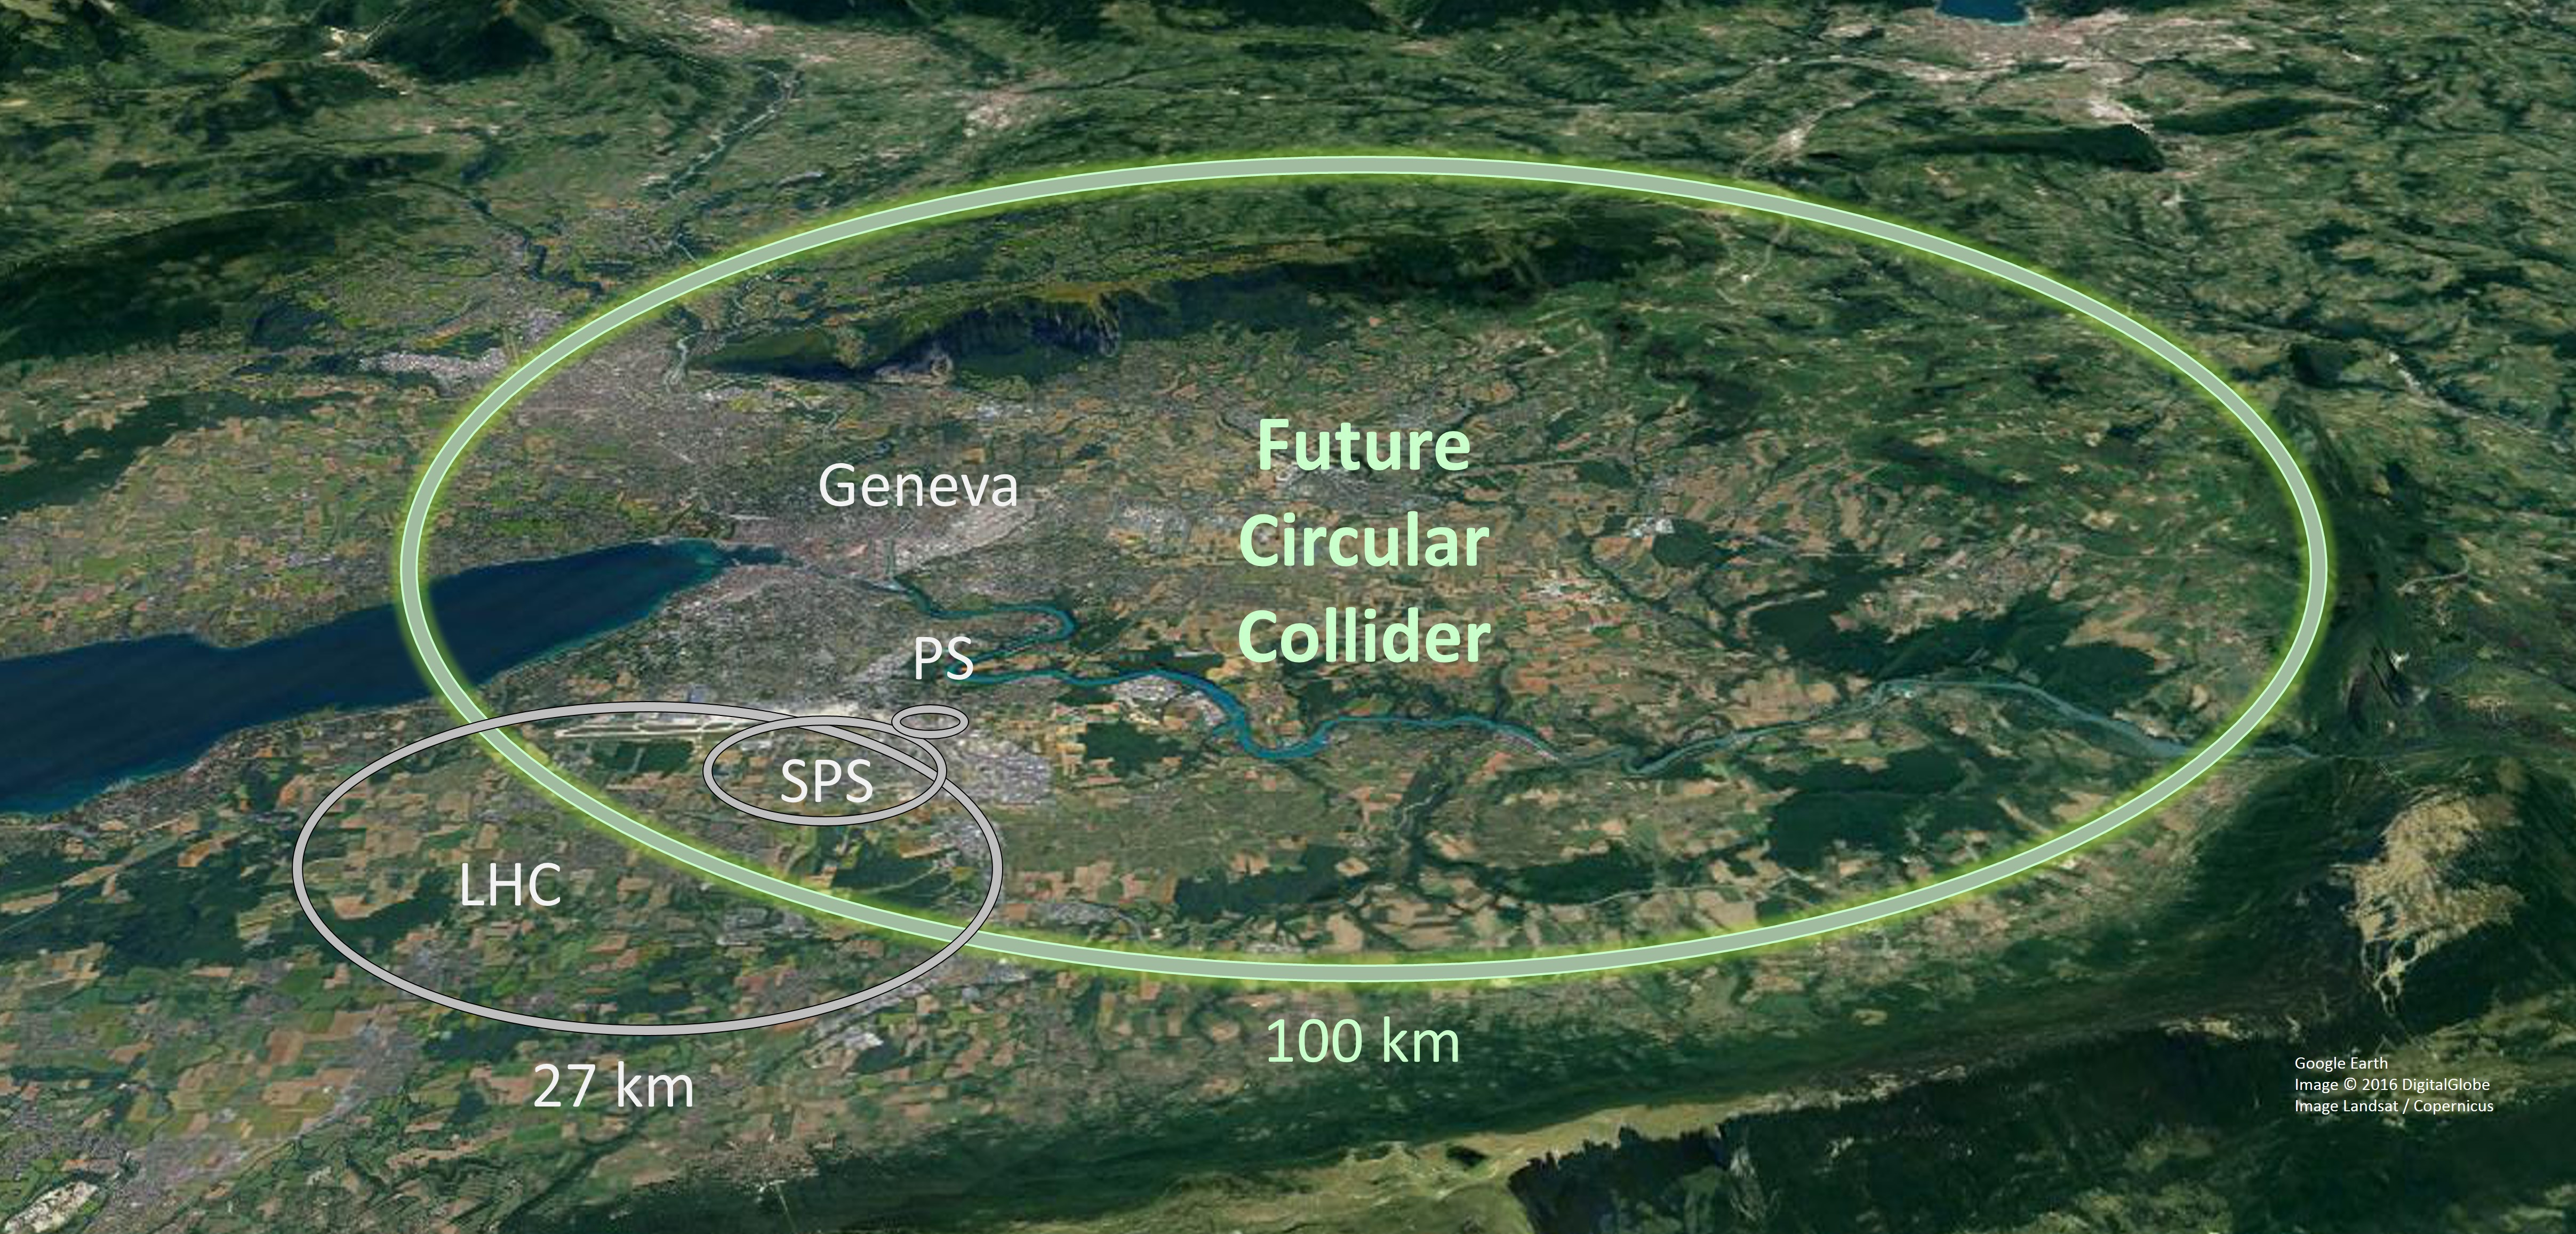
\includegraphics[width=\textwidth]{../img/FCC.jpg}
    \caption{https://cds.cern.ch/images/OPEN-PHO-ACCEL-2019-001-2}
    \label{fcc:img}
\end{figure}

Une fois encore, le détecteur SDHCAL candidate pour ce projet et pourrait être y être installer.

\section{Développement Numérique}

Mon objectif est d'adapter les codes développés précédemment par Guillaume 
\textsc{Garillot} du projet ILC au projet FCC qui n'utilise pas les mêmes suites logiciels.


\subsection{Programme : \convert}

Dans un premier temps, je dois convertir les fichiers \SLCIO en fichiers \ROOT en utilisant le programme libre \texttt{k4MarlinWrapper} du projet de \texttt{key4hep}\footnote{\url{https://github.com/key4hep/k4MarlinWrapper}}. 
Il s'agit d'une collaboration entre chercheurs du CERN dont l'objectif est de développer des outils pour le projet FCC, y compris des utils de conversion entre \LCIO (\iLCSoft) et \EDMhep (\FCC).%, en utilisant les algorithmes \texttt{Gaudi}
\\

Cette partie a été laborieux, car le programme \texttt{k4MarlinWrapper} est en cours de développement. 
J'ai du faire remonter de très nombreux problèmes en parallèle de mon travail. 
En effet, à chaque mise à jour, le programme ne fonctionnait plus, ce qui m'a fait perdre beaucoup de temps en essayant de comprendre le problème, le signaler et le corriger quand je le comprenais, ou patienter pour que quelqu'un d'autre le corrige. 

\subsection{Programme : \processor}

Comme les fichiers d'entrées sont à présent des fichiers \ROOT, il faut adapter cette partie pour que les fichiers de sortie soit les mêmes ou au moins équivalent.

\subsection{Programme : \analysis}

Cette partie reste inchangé par rapport à \ilcsoft.